\section{AGV Waiting-Time Fairness}
\label{sec:priority-wait-fairness}

We measured each vehicle's total wait at parking nodes and lift lobbies for
configurations A, B, B2, and C over seeds 1--10 (100 jobs and 20 AGVs per
seed). Each schedule was checked by the independent verifier; all plans
passed \cite{projectRepo}. The table reports the mean and standard deviation across the
ten per-seed fairness statistics. Pearson and Spearman correlations use the
fixed AGV priority rank (1 is highest); Gini is calculated over per-AGV total
wait. The max/min ratio is infinite whenever any AGV has zero wait.

\begin{table}[htbp]
\centering
\caption{Waiting fairness by configuration, mean $\pm$ standard deviation over ten seeds.}
\label{tab:fairness-configs}
% Generated by make_paper_numbers.py; do not edit.
\begin{tabular}{lrrrr}
\toprule
Configuration & Pearson $r$ & Spearman $\rho$ & Gini & Max/min wait \\
\midrule
A & $0.884\pm0.073$ & $0.886\pm0.074$ & $0.382\pm0.018$ & $\infty$ (10/10) \\
B & $0.961\pm0.041$ & $0.965\pm0.033$ & $0.354\pm0.016$ & $\infty$ (10/10) \\
B2 & $0.419\pm0.267$ & $0.425\pm0.264$ & $0.143\pm0.036$ & $3.842\pm1.468$ \\
C & $0.419\pm0.267$ & $0.425\pm0.264$ & $0.143\pm0.036$ & $3.842\pm1.468$ \\
\bottomrule
\end{tabular}

\end{table}

The figure plots mean total wait by fixed priority rank. A and B concentrate
delay strongly toward lower-priority ranks. B2 and C have identical wait
statistics in this experiment, consistent with their identical FCFS leg
ordering and schedules: the floor-server split itself did not change fairness
here. C reduces inequality relative to A and B (lower Gini and a smaller
priority-wait correlation), but the top-ranked AGV waits longer on average in
C (\WaitTopC~s) than under A or B (\WaitTopA~s in each). Thus the hybrid is fairer by
these aggregate distribution and rank-correlation measures, while shifting
some delay onto the highest-priority vehicle; this is not an unqualified
fairness improvement.

\begin{figure}[htbp]
\centering
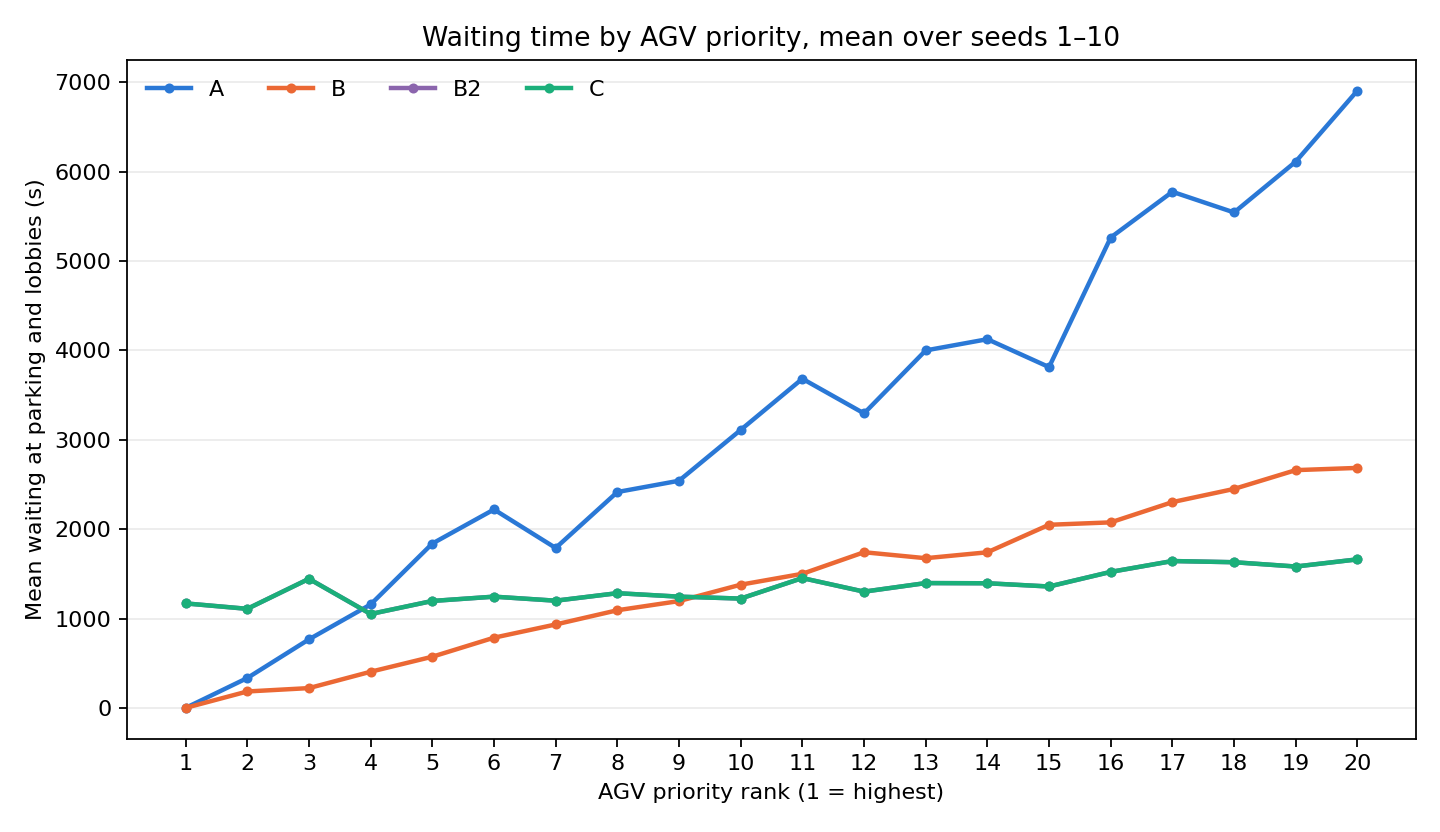
\includegraphics[width=0.9\linewidth]{../figures/mean_wait_by_priority.png}
\caption{Mean parking-plus-lobby wait by fixed AGV priority rank over seeds 1--10.}
\label{fig:wait-rank}
\end{figure}

\subsection{Fairness variants on C}

Two simple changes were evaluated on the same ten seeds. In the rotation
variant, job batches rotate the AGV priority ordering. In the waiting-trigger
variant, AGVs whose accumulated wait exceeded 600 s were promoted during
replanning; 600 s is a trigger, not a hard cap. All variant plans passed the
independent verifier.

\begin{table}[htbp]
\centering
\caption{C fairness variants: mean $\pm$ standard deviation over ten seeds.}
\label{tab:fairness-variants}
% Generated by make_paper_numbers.py; do not edit.
\begin{tabular}{lrrr}
\toprule
Variant & Makespan (s) & Tardiness (s) & Imbalance (s) \\
\midrule
C (baseline) & $2768.9\pm195.8$ & $90104.5\pm11447.3$ & $1441.2\pm241.1$ \\
C with rotating priority & $2737.6\pm169.7$ & $88009.6\pm10147.2$ & $1425.3\pm250.6$ \\
C with 600 s wait-trigger boost & $2768.9\pm195.8$ & $90104.5\pm11447.3$ & $1441.2\pm241.1$ \\
\bottomrule
\end{tabular}

\end{table}

Rotation lowered the reported mean makespan, tardiness and imbalance slightly,
but the Gini increased from \GiniC{} to \GiniCRotate{}; it weakened correlation with the
original fixed ranks but did not reduce overall wait inequality. The wait
trigger produced the same schedules and performance metrics as baseline C:
under the current FCFS leg order, priority changes mostly affect ties and did
not alter route-leg order. These results are descriptive for ten seeds; no
significance test was performed \cite{projectRepo}.

